% Created 2024-02-02 Fri 08:44
% Intended LaTeX compiler: pdflatex
\documentclass[presentation]{beamer}
\usepackage[utf8]{inputenc}
\usepackage[T1]{fontenc}
\usepackage{graphicx}
\usepackage{longtable}
\usepackage{wrapfig}
\usepackage{rotating}
\usepackage[normalem]{ulem}
\usepackage{amsmath}
\usepackage{amssymb}
\usepackage{capt-of}
\usepackage{hyperref}
\mode<beamer>{\usetheme{Madrid}}
\definecolor{SUred}{rgb}{0.59375, 0, 0.17969} % SU red (primary)
\definecolor{SUblue}{rgb}{0, 0.17578, 0.38281} % SU blue (secondary)
\setbeamercolor{palette primary}{bg=SUred,fg=white}
\setbeamercolor{palette secondary}{bg=SUblue,fg=white}
\setbeamercolor{palette tertiary}{bg=SUblue,fg=white}
\setbeamercolor{palette quaternary}{bg=SUblue,fg=white}
\setbeamercolor{structure}{fg=SUblue} % itemize, enumerate, etc
\setbeamercolor{section in toc}{fg=SUblue} % TOC sections
% Override palette coloring with secondary
\setbeamercolor{subsection in head/foot}{bg=SUblue,fg=white}
\setbeamercolor{date in head/foot}{bg=SUblue,fg=white}
\institute[SU]{Shenandoah University}
\titlegraphic{\includegraphics[width=0.5\textwidth]{\string~/Documents/suLogo/suLogo.pdf}}
\newcommand{\R}{\mathbb{R}}
\usepackage{tikz}
\usetheme{default}
\author{Chase Mathison\thanks{cmathiso@su.edu}}
\date{2 February 2024}
\title{The Other Trig Functions}
\hypersetup{
 pdfauthor={Chase Mathison},
 pdftitle={The Other Trig Functions},
 pdfkeywords={},
 pdfsubject={},
 pdfcreator={Emacs 29.1 (Org mode 9.6.7)}, 
 pdflang={English}}
\begin{document}

\maketitle

\section{Announcements}
\label{sec:orgbf5a172}
\begin{frame}[label={sec:orgd735532}]{Announcements}
\begin{enumerate}
\item Homework in M.O.M.
\item Quiz due tonight
\item Office hours today: 10am - 11am
\end{enumerate}
\end{frame}

\section{Lecture}
\label{sec:org68df652}
\begin{frame}[label={sec:org1b1051f}]{The Other Trig Functions}
\begin{columns}
\begin{column}{0.45\columnwidth}
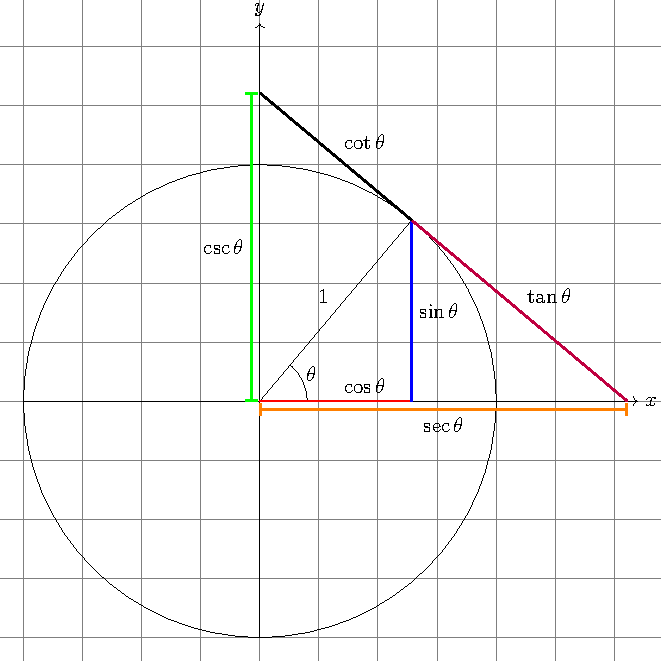
\includegraphics[width=\textwidth]{./circ.pdf}
\end{column}

\begin{column}{0.45\columnwidth}
\begin{block}{}
If \(\left( x,y \right)\) is the point on the unit circle associated with the
angle \(\theta\), then:
\begin{enumerate}
\item \(\tan(\theta) =\)
\item \(\cot(\theta) =\)
\item \(\sec(\theta) =\)
\item \(\csc(\theta) =\)
\end{enumerate}
\end{block}
\end{column}
\end{columns}
\end{frame}

\begin{frame}[label={sec:org298691e}]{Examples}
Find all of the trig functions evaluated at \(\theta = \frac{\pi}{6}\) radians.

\vspace{10in}
\end{frame}
\begin{frame}[label={sec:orgd7a1878}]{Examples}
Find all of the trig functions evaluated at \(\alpha = \frac{\pi}{4}\) radians.

\vspace{10in}
\end{frame}
\begin{frame}[label={sec:orgcb673ef}]{The Trig Functions in Quadrant I}
\begin{center}
\begin{tabular}{|l|ccccc|}
\hline
\(\theta\) & \(0\) & \(\frac{\pi}{6}\) & \(\frac{\pi}{4}\) & \(\frac{\pi}{3}\) & \(\frac{\pi}{2}\)\\[0pt]
 & or \(0^{\circ}\) &  &  &  & or \(90^{\circ}\)\\[0pt]
\hline
\(\sin(\theta)\) & \hspace{0.3in} & \hspace{0.3in} & \hspace{0.3in} & \hspace{0.3in} & \hspace{0.3in}\\[0pt]
 &  &  &  &  & \\[0pt]
\(\cos(\theta)\) &  &  &  &  & \\[0pt]
 &  &  &  &  & \\[0pt]
\(\tan(\theta)\) &  &  &  &  & \\[0pt]
 &  &  &  &  & \\[0pt]
\(\cot(\theta)\) &  &  &  &  & \\[0pt]
 &  &  &  &  & \\[0pt]
\(\sec(\theta)\) &  &  &  &  & \\[0pt]
 &  &  &  &  & \\[0pt]
\(\csc(\theta)\) &  &  &  &  & \\[0pt]
\hline
\end{tabular}
\end{center}
\end{frame}


\begin{frame}[label={sec:orge180022}]{Using Reference Angles}
To find the trig functions in the other quadrants, just remember to use reference angles
and that:
\textbf{A}ll \textbf{S}tudents \textbf{T}ake \textbf{C}alculus

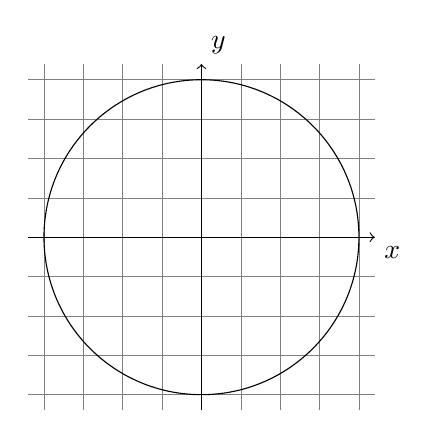
\begin{tikzpicture}[scale=2]
  \draw[help lines, step=0.25] (-1.1,-1.1) grid (1.1,1.1);
  \draw[->] (-1.1,0) -- (1.1,0) node [anchor=north west] {$x$};
  \draw[->] (0,-1.1) -- (0,1.1) node [anchor=south west] {$y$};
  \draw (0,0) circle [radius=1];
\end{tikzpicture}
\end{frame}

\begin{frame}[label={sec:orgc8c08e9}]{Example}
Find:
\begin{enumerate}
\item \(\sec(120^{\circ})\)
\item \(\csc\left(\frac{7\pi}{6}\right)\)
\item \(\tan\left(\frac{7\pi}{4}\right)\)
\item \(\cot(390^{\circ})\)
\end{enumerate}

\vspace{10in}
\end{frame}

\begin{frame}[label={sec:org108205a}]{Example}
\end{frame}

\begin{frame}[label={sec:orgd72816f}]{Even and Odd Functions}
\begin{columns}
\begin{column}{0.45\columnwidth}
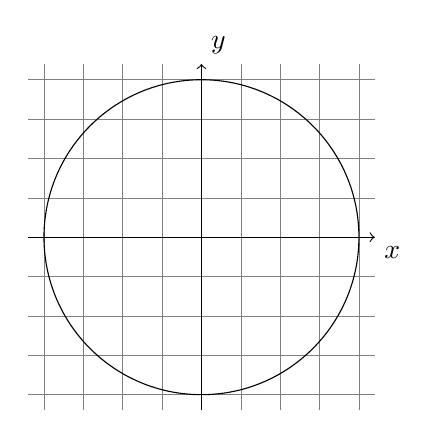
\begin{tikzpicture}[scale=2]
  \draw[help lines, step=0.25] (-1.1,-1.1) grid (1.1,1.1);
  \draw[->] (-1.1,0) -- (1.1,0) node [anchor=north west] {$x$};
  \draw[->] (0,-1.1) -- (0,1.1) node [anchor=south west] {$y$};
  \draw (0,0) circle [radius=1];
\end{tikzpicture}
\end{column}

\begin{column}{0.45\columnwidth}
\begin{block}{Even and Odd Functions}
A function \(f(x)\) is called \uline{\hspace*{1in}} if \(f(-x) = f(x)\).

A function \(f(x)\) is called \uline{\hspace*{1in}} if \(f(-x) = -f(x)\).

The following trig functions are even:
\vspace{0.5in}

The following trig functions are odd:
\vspace{0.5in}
\end{block}
\end{column}
\end{columns}
\end{frame}

\begin{frame}[label={sec:org7efe96b}]{Example}
Suppose \(\cos(\beta) = \frac{3}{7}.\) Then what is \(\cos(-\beta)?\)
\vspace{10in}
\end{frame}

\begin{frame}[label={sec:orgac30275}]{Fundamental Identities}
It's important to recognize how the trig functions are all related to
each other: They really are all based off of \(\sin(\theta)\) and \(\cos(\theta)\)!

\begin{block}{Fundamental Identities}
\vspace*{0.2in}
\begin{enumerate}
\item \(\tan\theta = \frac{\hspace{1in}}{\hspace{1in}}\)\vspace*{0.2in}
\item \(\cot\theta = \frac{\hspace{1in}}{\hspace{1in}}\)\vspace*{0.2in}
\item \(\sec\theta = \frac{\hspace{1in}}{\hspace{1in}}\)\vspace*{0.2in}
\item \(\csc\theta = \frac{\hspace{1in}}{\hspace{1in}}\)\vspace*{0.2in}
\end{enumerate}
\end{block}
\end{frame}

\begin{frame}[label={sec:org1d3331b}]{Example}
Suppose \(\sin(\gamma) = \frac{1}{3}\), and \(\frac{\pi}{2} \le
\gamma \le \pi\).  Find the other 6 trig functions at \(\gamma\).
\vspace{10in}
\end{frame}

\begin{frame}[label={sec:orgf4f66b4}]{Example}
\end{frame}

\begin{frame}[label={sec:org28da791}]{Example}
Suppose \(\sec(\theta) = -10\) and \(\pi \le \theta \le
\frac{3\pi}{2}.\) Find the other 6 trig functions at \(\theta\).
\vspace{10in}
\end{frame}
\end{document}